% !TeX spellcheck = fr-toutesvariantes
\documentclass[12pt]{report}
\usepackage{longtable}
\usepackage[table,xcdraw]{xcolor}
\usepackage[utf8]{inputenc}
\usepackage[T1]{fontenc}
\usepackage[francais]{babel}
\usepackage{fixltx2e}
\usepackage{charter}
\usepackage{amsmath}
\usepackage{float}
\usepackage{wrapfig}
\usepackage{graphicx}
\usepackage{soul}
\usepackage[colorlinks=true, linkcolor=blue]{hyperref}
\usepackage{parskip}
\usepackage{enumitem}
\usepackage[final]{pdfpages}
\usepackage[linguistics]{forest}
%\usepackage{titlesec}
\usepackage{listings}
\usepackage[final]{pdfpages}
\usepackage[=small,labelfont=bf]{caption} % Required for specifying captions to tables and figures
\usepackage[linesnumbered,algoruled,french,onelanguage]{algorithm2e}
\usepackage{url}
\usepackage{amsmath}
\usepackage{algorithmicx}
\usepackage{xcolor}
\usepackage{multirow}
\usepackage[noend]{algpseudocode}
\usepackage{tabularx}  % for tabularx
% to make cells in table have decent spacing
\usepackage{diagbox}
\usepackage{color, colortbl}
\usepackage{array}
\usepackage{tabularx} % in the preamble
\usepackage{csvsimple}
\usepackage{geometry}
\geometry{
	a4paper,
	total={170mm,257mm},
	left=20mm,
	top=20mm,
}
\usepackage{wrapfig}

\newcolumntype{L}[1]{>{\raggedright\let\newline\\\arraybackslash\hspace{0pt}}m{#1}}
\newcolumntype{C}[1]{>{\centering\let\newline\\\arraybackslash\hspace{0pt}}m{#1}}
\newcolumntype{R}[1]{>{\raggedleft\let\newline\\\arraybackslash\hspace{0pt}}m{#1}}

\def \hfillx {\hspace*{-\textwidth} \hfill}
\definecolor{Magenta}{RGB}{255,0,255}





\begin{document}
\hypersetup{hidelinks}

\includepdf[pages=1]{Page_garde.pdf} 
\tableofcontents

\pagenumbering{arabic}
\newpage


\part{Système expert et modèle d'inférence}
\chapter{Introduction}
\section{Problématique et besoins}
\section{Définitions}
\subsection{Règles de production}
\subsection{Moteur d'inférence}
\subsection{Système expert}

\chapter{Implémentation d'un système expert en Java}
\section{Outils utilisés}\label{usedTools}
\subsection{Langage de programmation : }
\paragraph{}
Nous avons opté pour le langage \href{https://fr.wikipedia.org/wiki/Java_(technique)}{Java}, car il offre une grande flexibilité et facilite l'implémentation qui est due au fait qu'il soit totalement orienté-objet.
\subsection{IDE : }
\paragraph{IntelliJ Idea} L'environnement de développement choisit est \href{https://www.jetbrains.com/idea/}{IntelliJ IDEA}, spécialement dédié au développement en utilisant le langage \href{https://fr.wikipedia.org/wiki/Java_(technique)}{Java}. Il est proposé par l'entreprise \href{https://www.jetbrains.com}{JetBrains} et est caractérisé par sa forte simplicité d'utilisation et les nombreux plugins et extensions qui lui sont dédiées.
\section{Analyseur de règles de production}
\paragraph{}
Afin de minimiser la modification du code, et pour des soucis de gain de temps, nous avons implémenter un mini-analyseur dont le but est de charger le contenu de deux fichiers(variables,rules) dans la base de faits d'un expert, le format adopté est inspiré des langages balisés, ce module se compose de sous modules : \\
\subsection{Analyseur de variables (variableParser)} \label{varParser}
\paragraph{}
Il s'occupe de prendre en entré un fichier remplit avec des variables et leurs valeurs possible(dans langage que nous avons mis au point), toute variable est de la forme suivante : \\
\newpage
\begin{minipage}{\textwidth}
	\centering
	\Large{<\textcolor{blue}{VarName} : \textcolor{Magenta}{Type}>val$_1$,$\dots$,val$_n$,</\textcolor{blue}{VarName}>}
\end{minipage}
\\
\begin{itemize}[label=\textbullet, font=\color{black}]
	\item La liste de valeurs possibles val$_1$,$\dots$,val$_n$, peut être vide.
	\item \textcolor{blue}{VarName} est le nom de la variable qui servira à l'identifier plus tard dans le programme.
	\item \textcolor{Magenta}{Type} est une structure que nous avons conçu pour supporter entre autre les type primitifs : String,Int,Double.. mais aussi les intervalles([a,b],]a,b],[$-\infty$,b]$\dots$) 	
\end{itemize}

\paragraph{}Quelques examples de variables : \\
\begin{itemize}[label=\textbullet, font=\color{black}]
	\item <\textcolor{blue}{Season} : \textcolor{Magenta}{String}>Summer,Winter,Autumn,Spring,</\textcolor{blue}{Season} >
	\item <\textcolor{blue}{Temperature} : \textcolor{Magenta}{Double}>28.5 , 15.5,</\textcolor{blue}{Temperature} >
	\item <\textcolor{blue}{Price} : \textcolor{Magenta}{Double}></\textcolor{blue}{Temperature} >
\end{itemize}

\subsection{Analyseur de règles (ruleParser)} 
\paragraph{}
Ce module prend en entré un fichier de règles écrite elles aussi dans une langage dédié, toute règle s'écrit comme suit : \\\\
\begin{minipage}{\textwidth}
	\centering
	\Large <VarResult> = <cond$_1$>, $\dots$ <cond$_n$>,\\
\end{minipage}

\paragraph{}Ou VarResult et cond$_i$ ont la même structure suivante : \\

\begin{minipage}{\textwidth}
	\centering
	\Large{<\textcolor{blue}{VarName}/\textcolor{Magenta}{Type}/\textcolor{gray}{cond}/\textcolor{red}{value}>}
\end{minipage}
\\
\begin{itemize}[label=\textbullet, font=\color{black}]
	\item \textcolor{blue}{VarName} est le nom de la variable qui servira à l'identifier plus tard dans le programme.
	\item \textcolor{Magenta}{Type} est le même type structuré vu dans \ref{varParser}
	\item \textcolor{gray}{cond} est la condtion sur la valeur de la variable courante(= ,< , > != ..)
	\textcolor{red}{value} La valeur suivant le type de la variable
\end{itemize}
\section{Modifications apportées}
\paragraph{}
Le système expert de base qui nous a été demandé d'améliorer était très limité(gère les valeurs comme des chaines de caractères uniquement, conditions d'égalité seulement entre les valeurs, ..), nous avons donc décidé d'ajouter certaines fonctionnalités a ce systèmes : \\
\subsection{Typage des variables}
L'inconvénient en travaillant seulement avec des String est le manque de flexibilité des valeurs, nous avons donc subdivisé le typage en 4 groupes : \\
\begin{itemize}[label=\textbullet, font=\color{black}]
	\item \textbf{StringVariableValue} : Type basique, généralement la plus part des variables ont ce type, il peut désigner un catégorie, un nom, une propriété nominale ... etc.
	\item \textbf{IntegerVariableValue} : Type basique pour désigner les valeurs discrètes telle que le nombre l'age.
	\item \textbf{DoubleVariableValue} : Type basique pour désigner les valeurs continues(beaucoup plus fréquentes) telles que le prix, la température ... etc
	\item \textbf{IntervalUnion} : Type complexe pour désigner tout séquence de valeur non dénombrable comme l'union de plusieurs intervalles([0,2]$\cup$[5,22]$\cup$[55,69[), une valeur minimum(value>min) our maximum ... etc
\end{itemize}

\subsection{Introduction de nouvelles conditions}
Les conditions utilisables n'étant que l'égalité et l'inégalité(qui ne fonctionnait pas à la base), nous avons opté pour une restructuration du système d'évaluation, avec l'introduction du typage vu précédemment nous avons pu introduire deux nouveaux opérateur de conditions qui sont le $>(\geq) $ et le $<(\leq)$, ces deux opérateur nous ont permis ainsi de délimiter sous forme d'intervalle les valeurs de certaines variables. 
\section{Interface modifié}
\paragraph{}
L'interface de base n'étant pas appropriée à notre besoin, nous avons décide de la modifier et la rendre adaptée au domaine choisi, plus de détails seront donnée dans la partie suivante
\section{Conclusion}
\paragraph{}
Les systèmes experts malgré leur simplicité ont prouvé leur efficacité durant les débuts de l'IA, cependant leur manque d'autonomie et de réaction avec le monde extérieur restait encore un obstacle majeur pour atteindre un niveau d'intelligence semblable à celui de l'homme, une extensions des systèmes expert à donc était développée, appelé système à agent-intelligents.
\part{Système multi-agents dans le domaine commercial }
\chapter{Introduction}
\section{Problématique}
\paragraph{}
Nous voudrions construire un système dans lequel il existe plusieurs vendeurs et plusieurs centres de ventes. Chaque vendeur propose ses produits en ligne, les centres de ventes à leur tour après avoir reçu une requête d’un acheteur, contactent les vendeurs suspectés d’avoir le produit recherché et retourne le résultat à l’utilisateur. Par exemple: 

On peut avoir les centres suivants:
\begin{itemize}
	\item Centre de vente d’appareil électronique.
	\item Centre de vente de vêtements.
\end{itemize}
Les vendeurs:
\begin{itemize}
	\item Vendeur de chaussures.
	\item Vendeur de téléphone portable.
	\item Vendeur de pantalon.
	\item Vendeur d’ordinateur.
\end{itemize}
On remarque que les centres sont caractérisés par une catégorie générale tandis que les vendeurs sont typiquement plus spécialisé dans un domaine donné, l’avantage de cette méthode est que l’utilisateur ne se soucie pas de la recherche du vendeur qui possède le produit recherché. Il va directement poser sa requête auprès d’un centre de ventes, et c’est à ce dernier de chercher le produit chez les vendeurs. Dans l’exemple précédent si le centre de vente d’appareil électronique reçoit une requête recherchant un ordinateur portable avec des paramètres donnés. Il va directement contacté le ou les vendeurs susceptible d’avoir le produit recherché, et donc le vendeur d’ordinateur.

Les vendeurs eux aussi n’ont pas à s’enregistrer chez les centres de ventes. Ils seront intelligemment contactés par ces derniers lors du traitement d’une requête donnée.\\
Pour réaliser un tel système de ventes nous allons nous baser sur un système multi-agents pour gérer la communication entre les centres de ventes et les vendeurs, ainsi que le traitement intelligent des requêtes des utilisateurs.
\section{Définitions}
\subsection{Agent intelligent}
\subsection{Système multi-agents}


% !TeX spellcheck = en_US
\chapter{Implémentation d'un système multi-agents avec la plateforme JADE}
\section{Outils utilisés}
\section{Schéma globale}
\paragraph{}
Notre conception du système multi-agents se base sur trois types d’agents:

Agent central: c’est l’agent qui s’occupe de la gestion des centres de ventes, il reçoit les requêtes des utilisateurs, après traitement il leur retourne les produits qu’ils cherchent.

Agent annexe: représente les vendeurs. Il reçoit une requête de l’agent central et il lui remet les produits présents dans sa base de données qui correspondent  à la requête.

Agent enregistreur: c’est l’agent qui garde les informations sur les différents agents centraux et annexes.
\newpage
\subsection{Agent annexe}
\paragraph{}
L’agent annexe se charge non seulement de répondre aux requêtes émises  par les centres de ventes mais aussi d’inférer des attributs à partir des informations de la requête pour mieux répondre à cette dernière.

Chaque agent annexe a une liste de règles qui permettent à un système expert de savoir si cet agent peut posséder un produit donnée.
\begin{figure}[H]
	\centering
	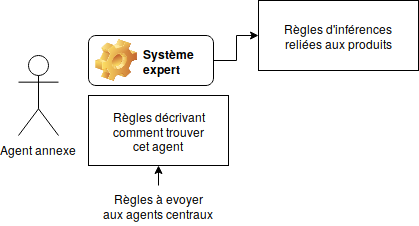
\includegraphics[scale=0.75]{imgs/annexeAgent.png}
	\caption{Illustration de l'agent annexe}
	\label{fig:annexeAgent}
\end{figure}

\subsection{Agent central}
\paragraph{}
L’agent central reçoit d’abord les règles des agents annexes afin qu’il puissent par la suite les contacter après avoir reçu une requête de l’utilisateur.
\begin{figure}[H]
	\centering
	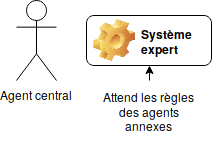
\includegraphics[scale=0.75]{imgs/centralAgent.png}
	\caption{Illustration de l'agent central}
	\label{fig:centralAgent}
\end{figure}


\section{Communication entre les agents}
La communication entre les agents se devise en deux parties principales:
\begin{itemize}
	\item Communication d’ajout de service.
	\item Communication de requête.
\end{itemize}
\subsection{Communication d'ajout de service}
Ce type de communication est principalement géré par l’agent enregistreur. Tout agent qui arrive dans le système devra  informer un agent enregistreur pour qu’il puissent garder ses informations.
\begin{figure}[H]
	\centering
	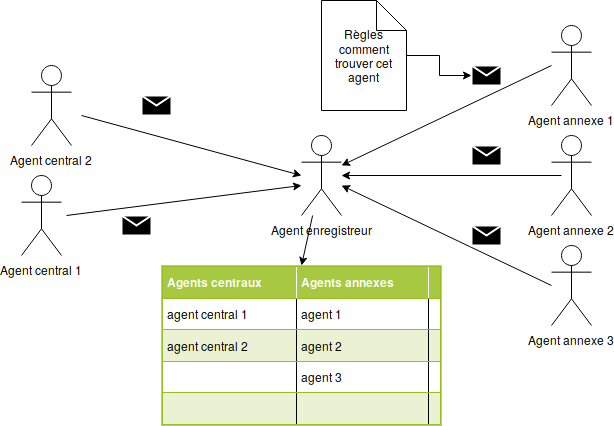
\includegraphics[scale=0.6]{imgs/comReg.png}
	\caption{Enregistrement des agents}
	\label{fig:registrations}
\end{figure}
Par la suite, l’agent enregistreur répond aux agents centraux et il leur communique les règles concernant les agents annexes afin qu’ils puissent les trouver lors de l’arriver d’une requête utilisateur.
\begin{figure}[H]
	\centering
	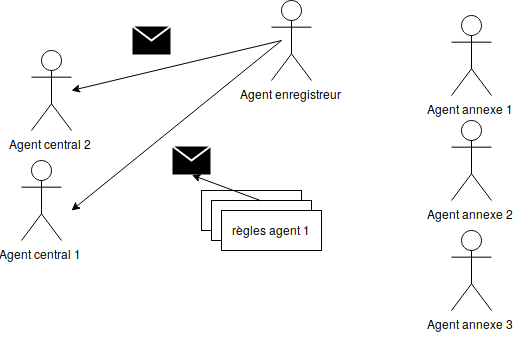
\includegraphics[scale=0.6]{imgs/sendRules.png}
	\caption{Enregistrement des agents}
	\label{fig:comRules}
\end{figure}
\newpage
Jusqu’à présent le vrai rôle de l’agent enregistreur n’apparait pas. C’est quand un nouveau agent qui se connecte dans le système qu’on aperçoit son rôle. Le nouveau agent n’a pas à communiquer avec tous les autres agents pour qu’il soit connu dans son environnement, il suffit d’informer l’agent enregistreur pour réaliser cela. Quand un agent annexe arrive, il envoi ses informations à l’agent enregistreur, ce dernier informe les agents centraux de son arrivé pour qu’ils puissent le contacter.
\begin{figure}[H]
	\centering
	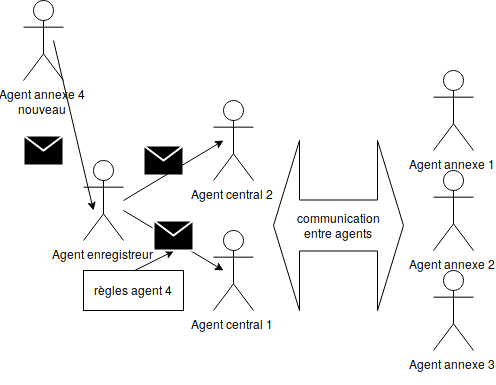
\includegraphics[scale=0.6]{imgs/newAnnexe.png}
	\caption{L'arrivé d'un nouveau agent annexe}
	\label{fig:newAnnexe}
\end{figure}
Quand un agent central arrive, l’agent enregistreur l’informe des agents annexes existant, et l’ajoute à la liste des agents centraux.
\begin{figure}[H]
	\centering
	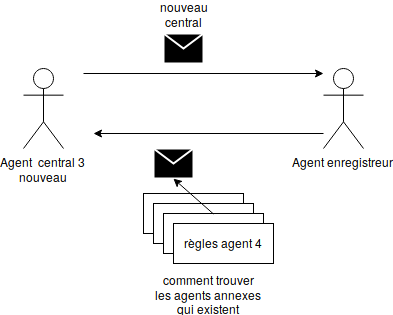
\includegraphics[scale=0.6]{imgs/newCentral.png}
	\caption{L'arrivé d'un nouveau agent central}
	\label{fig:newCentral}
\end{figure}
\newpage
\subsection{Communication de requêtes}
Ce type de communication concerne la partie des communications qui résulte de l’arriver d’une requête utilisateur. L’agent central qui reçoit la requête lance son moteur d’inférence pour déduire les agents susceptible d’avoir les produits spécifié par la requête. La requête est alors envoyer à ces agents pour qu’ils puissent y répondre.
\begin{figure}[H]
	\centering
	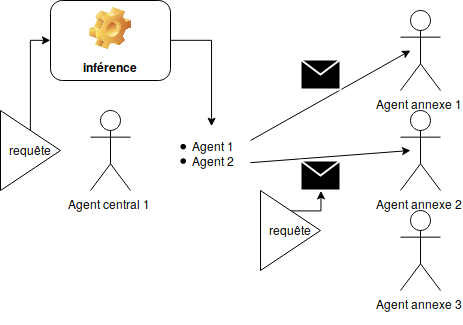
\includegraphics[scale=0.6]{imgs/annexeSelec.png}
	\caption{La sélection des agents annexes}
	\label{fig:annexeSelection}
\end{figure}
L'agent annexe qui reçoit la requête commence d’abord par essayer d’inférer de nouvelles connaissances sur le produit que l’utilisateur cherche. Ensuite il cherche dans sa base de données les produits qui correspondent à la requête. Le résultat obtenu est retourner à l’agent central pour qu’il les propose à l’acheteur.
\begin{figure}[H]
	\centering
	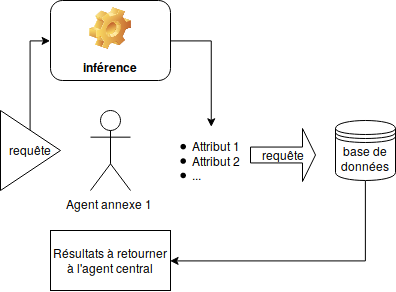
\includegraphics[scale=0.6]{imgs/annexeWork.png}
	\caption{Le travail d'un agent annexe}
	\label{fig:annexeWork}
\end{figure}

%amaze me here
\chapter{Application dédiée}
\section{Interface homme-machine}
\section{Conclusion}
\part{L'interpréteur JASON}
\setcounter{chapter}{0}
\chapter{Introduction}
\section{Problématique et besoins}
\paragraph{}
Durant la partie I, nous avons du concevoir nous même un moteur d'inférence utilisant le lange JAVA, cependant il serait plus intéressant de remplacer ce moteur basique par une moteur plus performant et plus adéquat aux système multi-agent, ce qui nous a amené a l'utilisation de la plateforme JASON.
\section{Définitions}
\subsection{Architecture CDI (Croyance-Désir-Intention)}
\paragraph{}
Une architecture BDI est conçue en partant du modèle "Croyance-Désir-Intention", en anglais "\textbf{Belief-Desire-Intention}", de la rationalité d'un agent intelligent. tel que les \textbf{croyances} sont les informations que l'agent possède sur l'environnement et sur d'autres agents qui existent dans le même environnement, les \textbf{désirs} représentent les états de l'environnement, et parfois de lui-même, que l'agent aimerait voir réalisés et finalement les \textbf{intentions} d'un agent sont les désirs que l'agent a décidé d'accomplir ou les actions qu'il a décidé de faire pour accomplir ses désirs( Même si tous les désirs d'un agent sont consistants, l'agent peut ne pas être capable d'accomplir tous ses désirs à la fois)
\subsection{AgentSpeakL}
\paragraph{}
AgentSpeak est un langage orienté agent. il est basé sur la programmation logique(Prolog) et les architectures CDI pour les agents cognitives.
\begin{figure}[H]
	\centering
	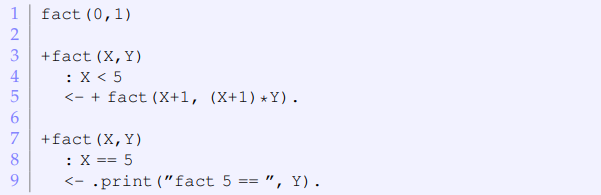
\includegraphics[width=\textwidth]{imgs/agenttSpeak.png}
	\caption{Exemple d'un agent voulant calculer le factoriel d'un nombre}
\end{figure}
\subsection{La plateforme JASON}
JASON est une plateforme qui a pour but de faciliter le développement de système multi-agent en offrant un environnement de travail complet comportant un éditeur de texte, un débogger et un compilateur AgentSpeak.
\chapter{Exemples de communication entre agents avec JASON}
\section{Environnement de travail}
\paragraph{}
L'IDE de la plateforme JASON est jEdit, il se présente comme tout IDE classique avec les fonctionnalités adéquates pour la manipulation des agents et des architectures BDI.
\begin{figure}[H]
	\centering
	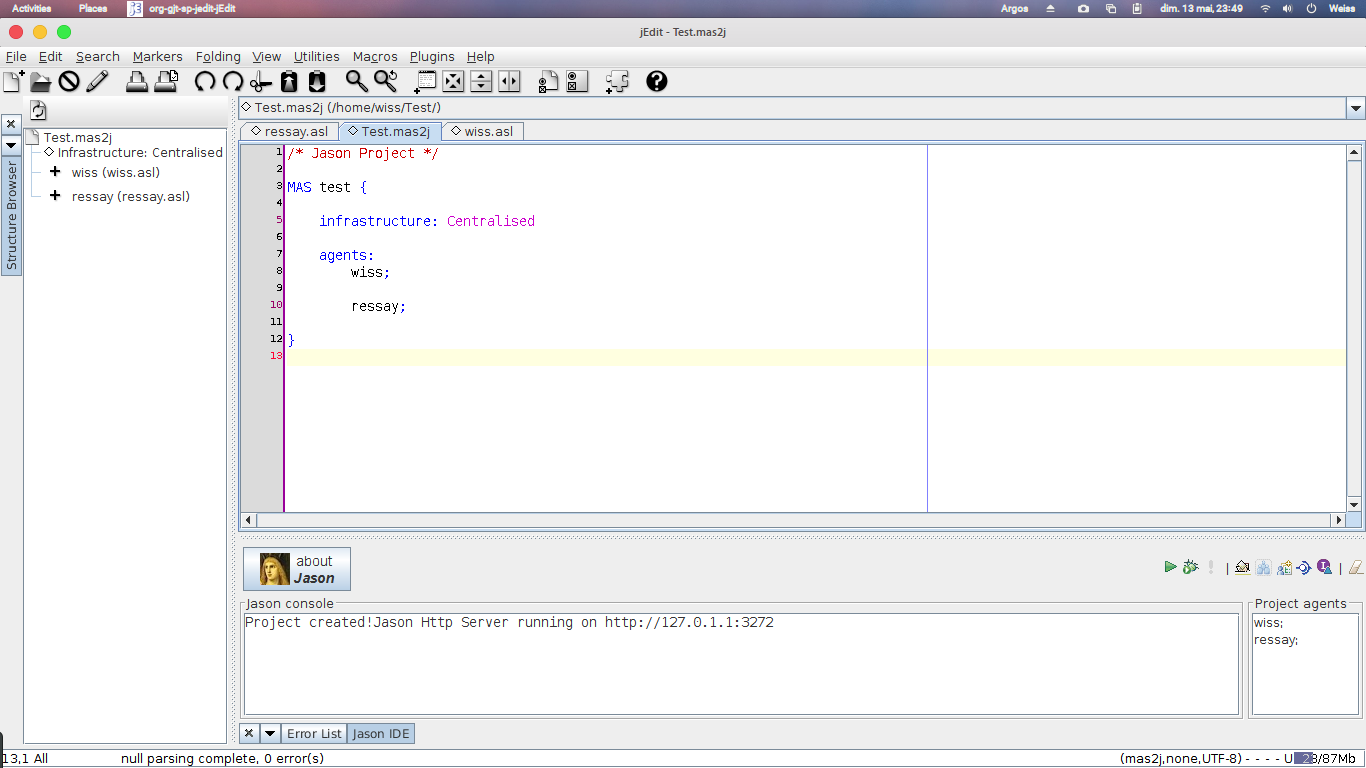
\includegraphics[width=\textwidth]{imgs/jEdit.png}
	\caption{Fenêtre d'édition de l'IDE jEdit}
\end{figure}
\newpage
\section{Inférence locale}
\paragraph{}
Un agent dans JASON peut utiliser l'architecture BDI pour lancer son propre moteur d'inférence, prenons l'exemple suivant : \\
\begin{itemize}[label=\textbullet]
	\item l'agent a une croyance initiale que la saison est l'été.
	\item il ajoutera la croyance article(tshirt) si la saison est l'été en exécutant le plan : sayTshirt.
\end{itemize}

\paragraph{}
le code est le suivant : \\
\begin{figure}[H]
	\centering
	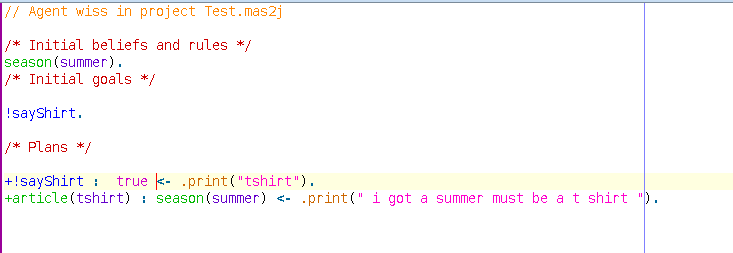
\includegraphics[width=0.8\textwidth]{imgs/jasonWiss.png}
	\caption{Code agentSpeak de l'agent wiss}
	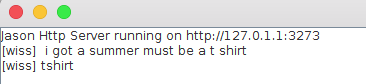
\includegraphics[width=0.8\textwidth]{imgs/jasonWissDone.png}
	\caption{résulat}
\end{figure}
\section{Scénario simple de communications}
\paragraph{}
Le scenario est le suivant : 
\begin{itemize}[label = \textbullet]
	\item l'agent Ressay envoie un message a l'agent Wiss lui disant que l'article est tshirt.
	\item l'agent Wiss attendra un message de la part de Ressay seulement car il l'a marqué comme étant fiable.
	\item Wiss ré-exécute l'inférence du scénario précédent.
\end{itemize}

\begin{figure}[H]
	\centering
	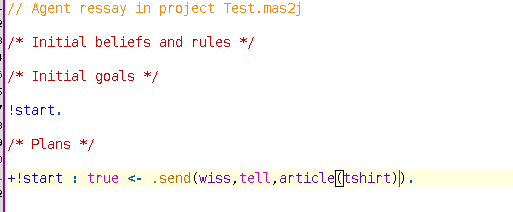
\includegraphics[width=0.8\textwidth]{imgs/jasonRessay.png}
	\caption{Ressay envoie le message}
	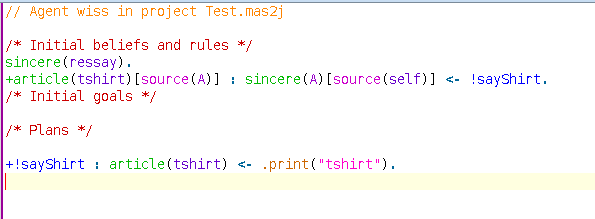
\includegraphics[width=0.8\textwidth]{imgs/wissRecievedRessay.png}
	\caption{Wiss reçoit}
	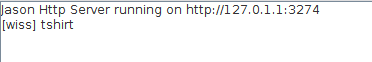
\includegraphics[width=0.8\textwidth]{imgs/wissRessayDone.png}
	\caption{Résultat}
	
\end{figure}

\chapter{Comparaison avec la plateforme JADE}
\section{Principales différence}
\section{Le critère de décision}
\input{chapter3Conclusion.tex}
\listoffigures
\listoftables
\bibliographystyle{abbrv}  
\bibliography{biblio.bib}
\input{appendix.tex}
\end{document}}\grid
